\documentclass[11pt,answers]{exam}

\usepackage{etex}
\usepackage{amssymb,amsmath,multicol} %<-- InWorksheetExam1 i also have fancyhdr,

\usepackage[metapost]{mfpic}
\usepackage[pdftex]{graphicx}
\usepackage{tabu}

\usepackage{pst-plot}
\usepackage{pgfplots}
\pgfplotsset{compat=1.9}

\usepackage{tikz}
\usepackage{tkz-2d}
\usepackage{tkz-base}
\usetikzlibrary{calc}
\usetikzlibrary{arrows}

\usepackage{systeme}

\usepackage[inline]{enumitem}
\usepackage{refcount}%<-- non in WorksheetExam1

\usepackage{pstricks-add,pst-eucl}
\usepackage{systeme}
\usepackage{setspace}
\usepackage{multicol}


\usepackage[inline]{enumitem}   
\makeatletter
% This command ignores the optional argument for itemize and enumerate lists
\newcommand{\inlineitem}[1][]{%
\ifnum\enit@type=\tw@
    {\descriptionlabel{#1}}
  \hspace{\labelsep}%
\else
  \ifnum\enit@type=\z@
       \refstepcounter{\@listctr}\fi
    \quad\@itemlabel\hspace{\labelsep}%
\fi}
\makeatother


\def\f{x+1} \def\g{-x/3+2}  \def\h{-x+3}

\newcommand{\vasymptote}[2][]{
    \draw [densely dashed,#1] ({rel axis cs:0,0} -| {axis cs:#2,0}) -- ({rel axis cs:0,1} -| {axis cs:#2,0});
}

\boxedpoints

\addpoints
%\printanswers
\noprintanswers

\opengraphsfile{Q11b_Fa18}

\begin{document}
\extrawidth{-0.3in}
\pagestyle{headandfoot}

\setlength{\hoffset}{-.25in}

\extraheadheight{-.3in}
\runningheadrule
\firstpageheader{\bfseries {Precalculus}}{ \bfseries {Quiz 11 }}{\bfseries {12/4/18}} 

\begin{center}
	This quiz has \numquestions\ questions, for a total of \numpoints\
	points and \numbonuspoints\ bonus points.
\end{center}


\firstpagefooter{} %%&&CHANGED
                {}
                {%Points earned: \hbox to 0.5in{\hrulefill}
                % out of  \pointsonpage{\thepage} points
                }
                 
						

\vspace*{0.1cm}
\hbox to \textwidth { \scshape {Name:} \enspace\hrulefill}
\vspace{0.1cm}




\pointpoints{point}{points}

\begin{questions}


\addpoints


 \question Part of the graph of a sinusoidal function  is shown below:
 
%%%%% \begin{mfpic}[35][50]{0}{5.25}{-1.15}{1.5}
%\point[3pt]{(1.5708,0), (2.3562,1), (3.1415,0), (3.927,-1), (4.7124,0)}
%%%%%\axes
%%%%%\tlabel[cc](5.25,-0.25){$x$}
%%%%%\tlabel[cc](0.25,1.5){$y$}
%%%%%\xmarks{1.5708, 2.3562, 3.1415, 3.927, 4.7124}
%%%%%\ymarks{-1,1}
%%%%%\tlpointsep{4pt}
%%%%%\axislabels {x}{{$\frac{\pi}{4}$} 0.7853, {$\frac{\pi}{2}$} 1.5708, {$\frac{3\pi}{4}$} 2.3562, {$\pi$} 3.1415, {$\frac{5\pi}{4}$} 3.927, {$\frac{3\pi}{2}$} 4.7124}
%%%%%\axislabels {y}{{$-1$} -1, {$1$} 1}
%%%%%\function{0, 4.7124, 0.1}{sin(4*x - 3.1415)} %1.5708
%%%%%\end{mfpic}


\begin{mfpic}[35]{-2}{2}{0}{3}

\point[3pt]{(1.5708,1.5), (0.7854,1), (0,1.5), (-0.7854,2), (-1.5708,1.5)}
\tlabel(-1.1,2.2){\tiny $\left(-\frac{\pi}{4},2\right )$}
\tlabel(0.55,0.75){\tiny $\left(\frac{\pi}{4},1\right )$}
\axes
\tlabel[cc](2,-0.25){\scriptsize $x$}
\tlabel[cc](0.25,3){\scriptsize $y$}
%\tcaption{\scriptsize One cycle  of $y = g(x)$.}
\xmarks{-1.5708,-0.7854,0.7854,1.5708}
\ymarks{1,2}
\tlpointsep{4pt}
\axislabels {x}{{\tiny $-\dfrac{\pi}{2} \hspace{7pt}$} -1.5708, {\tiny $-\dfrac{\pi}{4}\hspace{7pt}$} -0.7854, {\tiny $\dfrac{\pi}{4}$} 0.7854,  {\tiny $\dfrac{\pi}{2}$} 1.5708}
\axislabels {y}{ {\tiny $1$} 1, {\tiny $2$} 2}
\function{-1.5708, 1.5708, 0.1}{0.5*sin(3.14159+2*x)+1.5}
\end{mfpic}
 
 \begin{parts}
 	\part[1] The amplitude is: \hbox to 1in{\dotfill} 
 	\part[1] The period is: \hbox to 1in{\dotfill}
 	\bonuspart[1] The equation of the midline is: \hbox to 1in{\dotfill}
 	\part[2]  Write  an equation that represents the curve in the form
 	 $\displaystyle y = a \cos B(x - h)+k$. Show evidence of Your thinking, and write your equation in the space provided below.
 	
 	
 	\fillwithdottedlines{0.8in}
 	\medskip
 	
 	The equation is $y=$\dotfill
 	
 \end{parts}
 
 \question  Each time your heart beats, your blood pressure first increases and then decreases as the heart rests between beats. The maximum and minimum blood pressures are called the systolic and diastolic pressures, respectively. Your blood pressure reading is written as systolic/diastolic. A reading of 120/80 is considered normal. A certain person's blood pressure is modeled by the function
$\displaystyle p(t) = 130 + 25 \sin(150\pi t)$
where $p(t)$ is the pressure in mmHg (millimeters of mercury), at time $t$ measured in minutes.
\begin{parts}
	\part[2] Find the period of $p(t)$. Show evidence of Your thinking.
	\fillwithdottedlines{0.8in}
	\part[2] Find the person's maximum (systolic) blood pressure. Show evidence of Your thinking.
	\fillwithdottedlines{0.8in}
	\end{parts}
\end{questions}
\newpage

\par\medskip\hrule\medskip


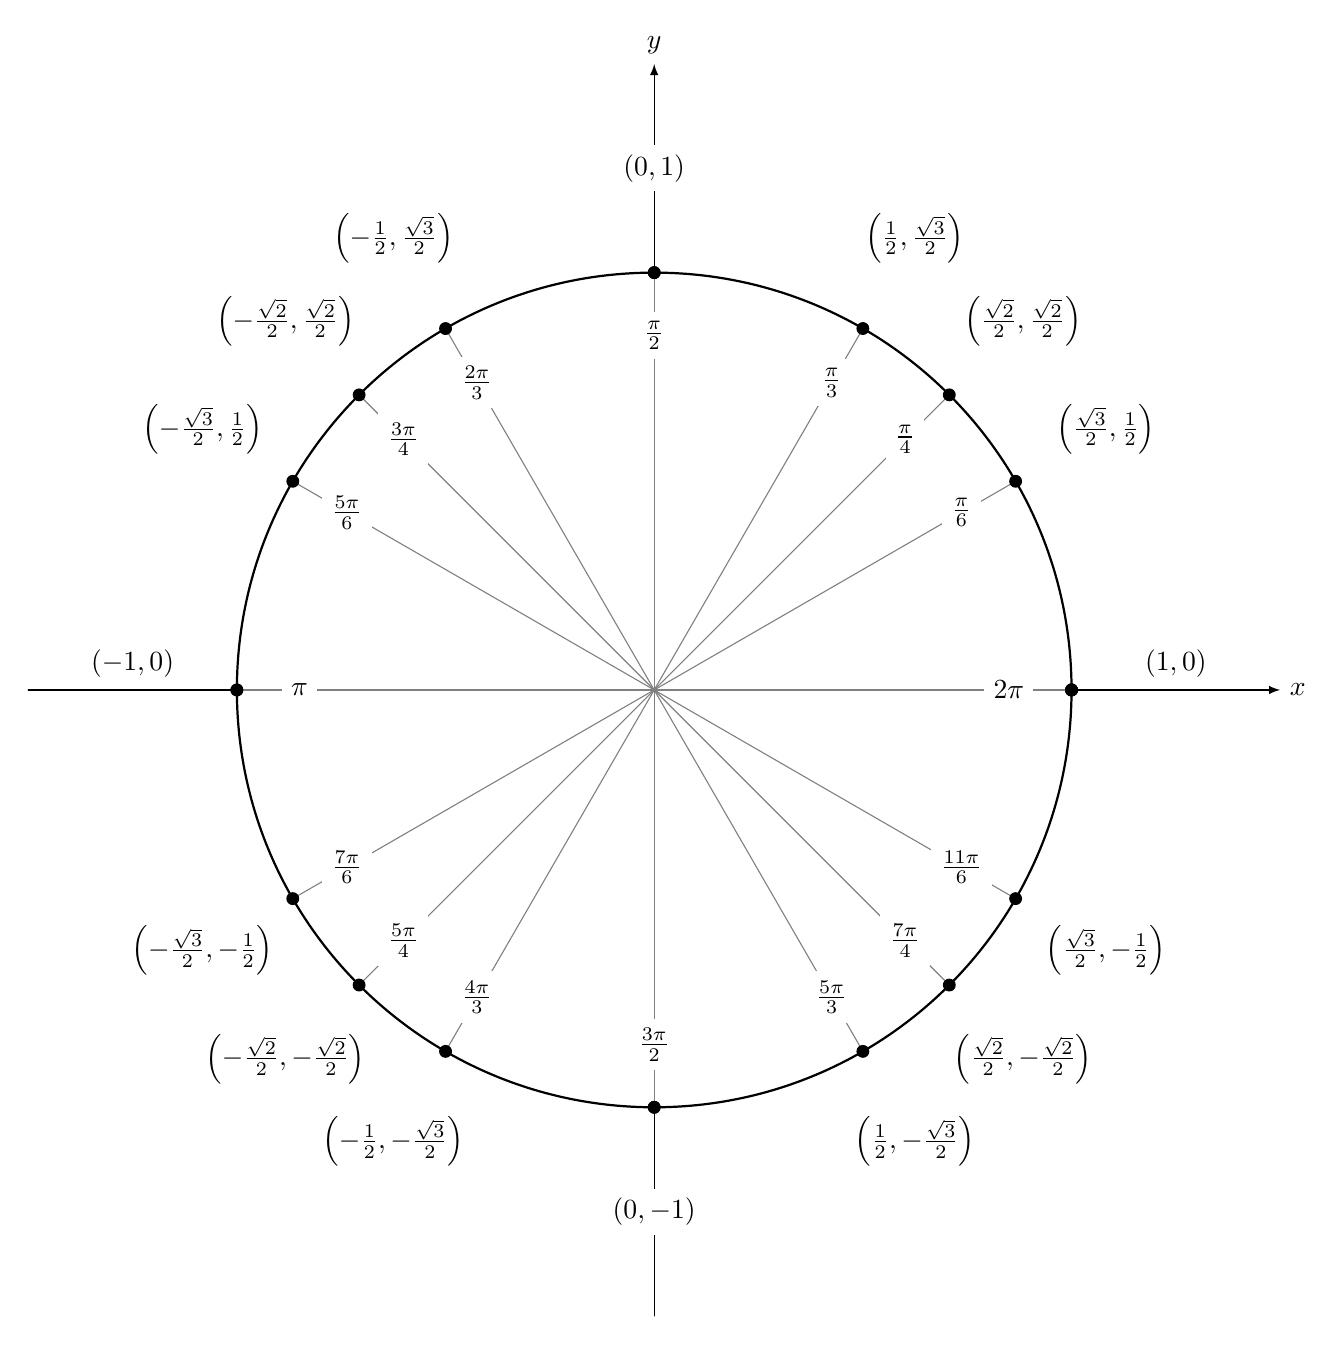
\begin{tikzpicture}[scale=5.3,cap=round,>=latex]
% draw the coordinates
\draw[->] (-1.5cm,0cm) -- (1.5cm,0cm) node[right,fill=white] {$x$};
\draw[->] (0cm,-1.5cm) -- (0cm,1.5cm) node[above,fill=white] {$y$};

% draw the unit circle
\draw[thick] (0cm,0cm) circle(1cm);

\foreach \x in {0,30,...,360} {
	% lines from center to point
	\draw[gray] (0cm,0cm) -- (\x:1cm);
	% dots at each point
	\filldraw[black] (\x:1cm) circle(0.4pt);
	% draw each angle in degrees
	%\draw (\x:0.6cm) node[fill=white] {$\x^\circ$};
}

\foreach \x in {0,45,...,360} {
	% lines from center to point
	\draw[gray] (0cm,0cm) -- (\x:1cm);
	% dots at each point
	\filldraw[black] (\x:1cm) circle(0.4pt);
	% draw each angle in degrees
	%\draw (\x:0.6cm) node[fill=white] {$\x^\circ$};
}
% draw each angle in radians
\foreach \x/\xtext in {
	30/\frac{\pi}{6},
	45/\frac{\pi}{4},
	60/\frac{\pi}{3},
	90/\frac{\pi}{2},
	120/\frac{2\pi}{3},
	135/\frac{3\pi}{4},
	150/\frac{5\pi}{6},
	180/\pi,
	210/\frac{7\pi}{6},
	225/\frac{5\pi}{4},
	240/\frac{4\pi}{3},
	270/\frac{3\pi}{2},
	300/\frac{5\pi}{3},
	315/\frac{7\pi}{4},
	330/\frac{11\pi}{6},
	360/2\pi}
\draw (\x:0.85cm) node[fill=white] {$\xtext$};

\foreach \x/\xtext/\y in {
	% the coordinates for the first quadrant
	30/\frac{\sqrt{3}}{2}/\frac{1}{2},
	45/\frac{\sqrt{2}}{2}/\frac{\sqrt{2}}{2},
	60/\frac{1}{2}/\frac{\sqrt{3}}{2},
	% the coordinates for the second quadrant
	150/-\frac{\sqrt{3}}{2}/\frac{1}{2},
	135/-\frac{\sqrt{2}}{2}/\frac{\sqrt{2}}{2},
	120/-\frac{1}{2}/\frac{\sqrt{3}}{2},
	% the coordinates for the third quadrant
	210/-\frac{\sqrt{3}}{2}/-\frac{1}{2},
	225/-\frac{\sqrt{2}}{2}/-\frac{\sqrt{2}}{2},
	240/-\frac{1}{2}/-\frac{\sqrt{3}}{2},
	% the coordinates for the fourth quadrant
	330/\frac{\sqrt{3}}{2}/-\frac{1}{2},
	315/\frac{\sqrt{2}}{2}/-\frac{\sqrt{2}}{2},
	300/\frac{1}{2}/-\frac{\sqrt{3}}{2}}
\draw (\x:1.25cm) node[fill=white] {$\left(\xtext,\y\right)$};

% draw the horizontal and vertical coordinates
% the placement is better this way
\draw (-1.25cm,0cm) node[above=1pt] {$(-1,0)$}
(1.25cm,0cm)  node[above=1pt] {$(1,0)$}
(0cm,-1.25cm) node[fill=white] {$(0,-1)$}
(0cm,1.25cm)  node[fill=white] {$(0,1)$};
\end{tikzpicture}



\end{document}                 